\documentclass[12pt,a4paper,oneside]{article}
\usepackage[colorlinks=true]{hyperref}
\usepackage[utf8]{inputenc}
\usepackage[czech]{babel}
\usepackage{graphicx}
\usepackage{pdfpages}
\textwidth 16cm \textheight 25cm
\topmargin -1.3cm 
\oddsidemargin 0cm
\pagestyle{empty}
\begin{document}
\title{Radiová meteorická detekční stanice RMDS01A}
\author{Jakub Kákona, kaklik@mlab.cz }
\maketitle

\begin{abstract}
Konstrukce základního softwarově definovaného přijímacího systému pro detekci meteorů.
\end{abstract}

\begin{figure} [htbp]
\begin{center}
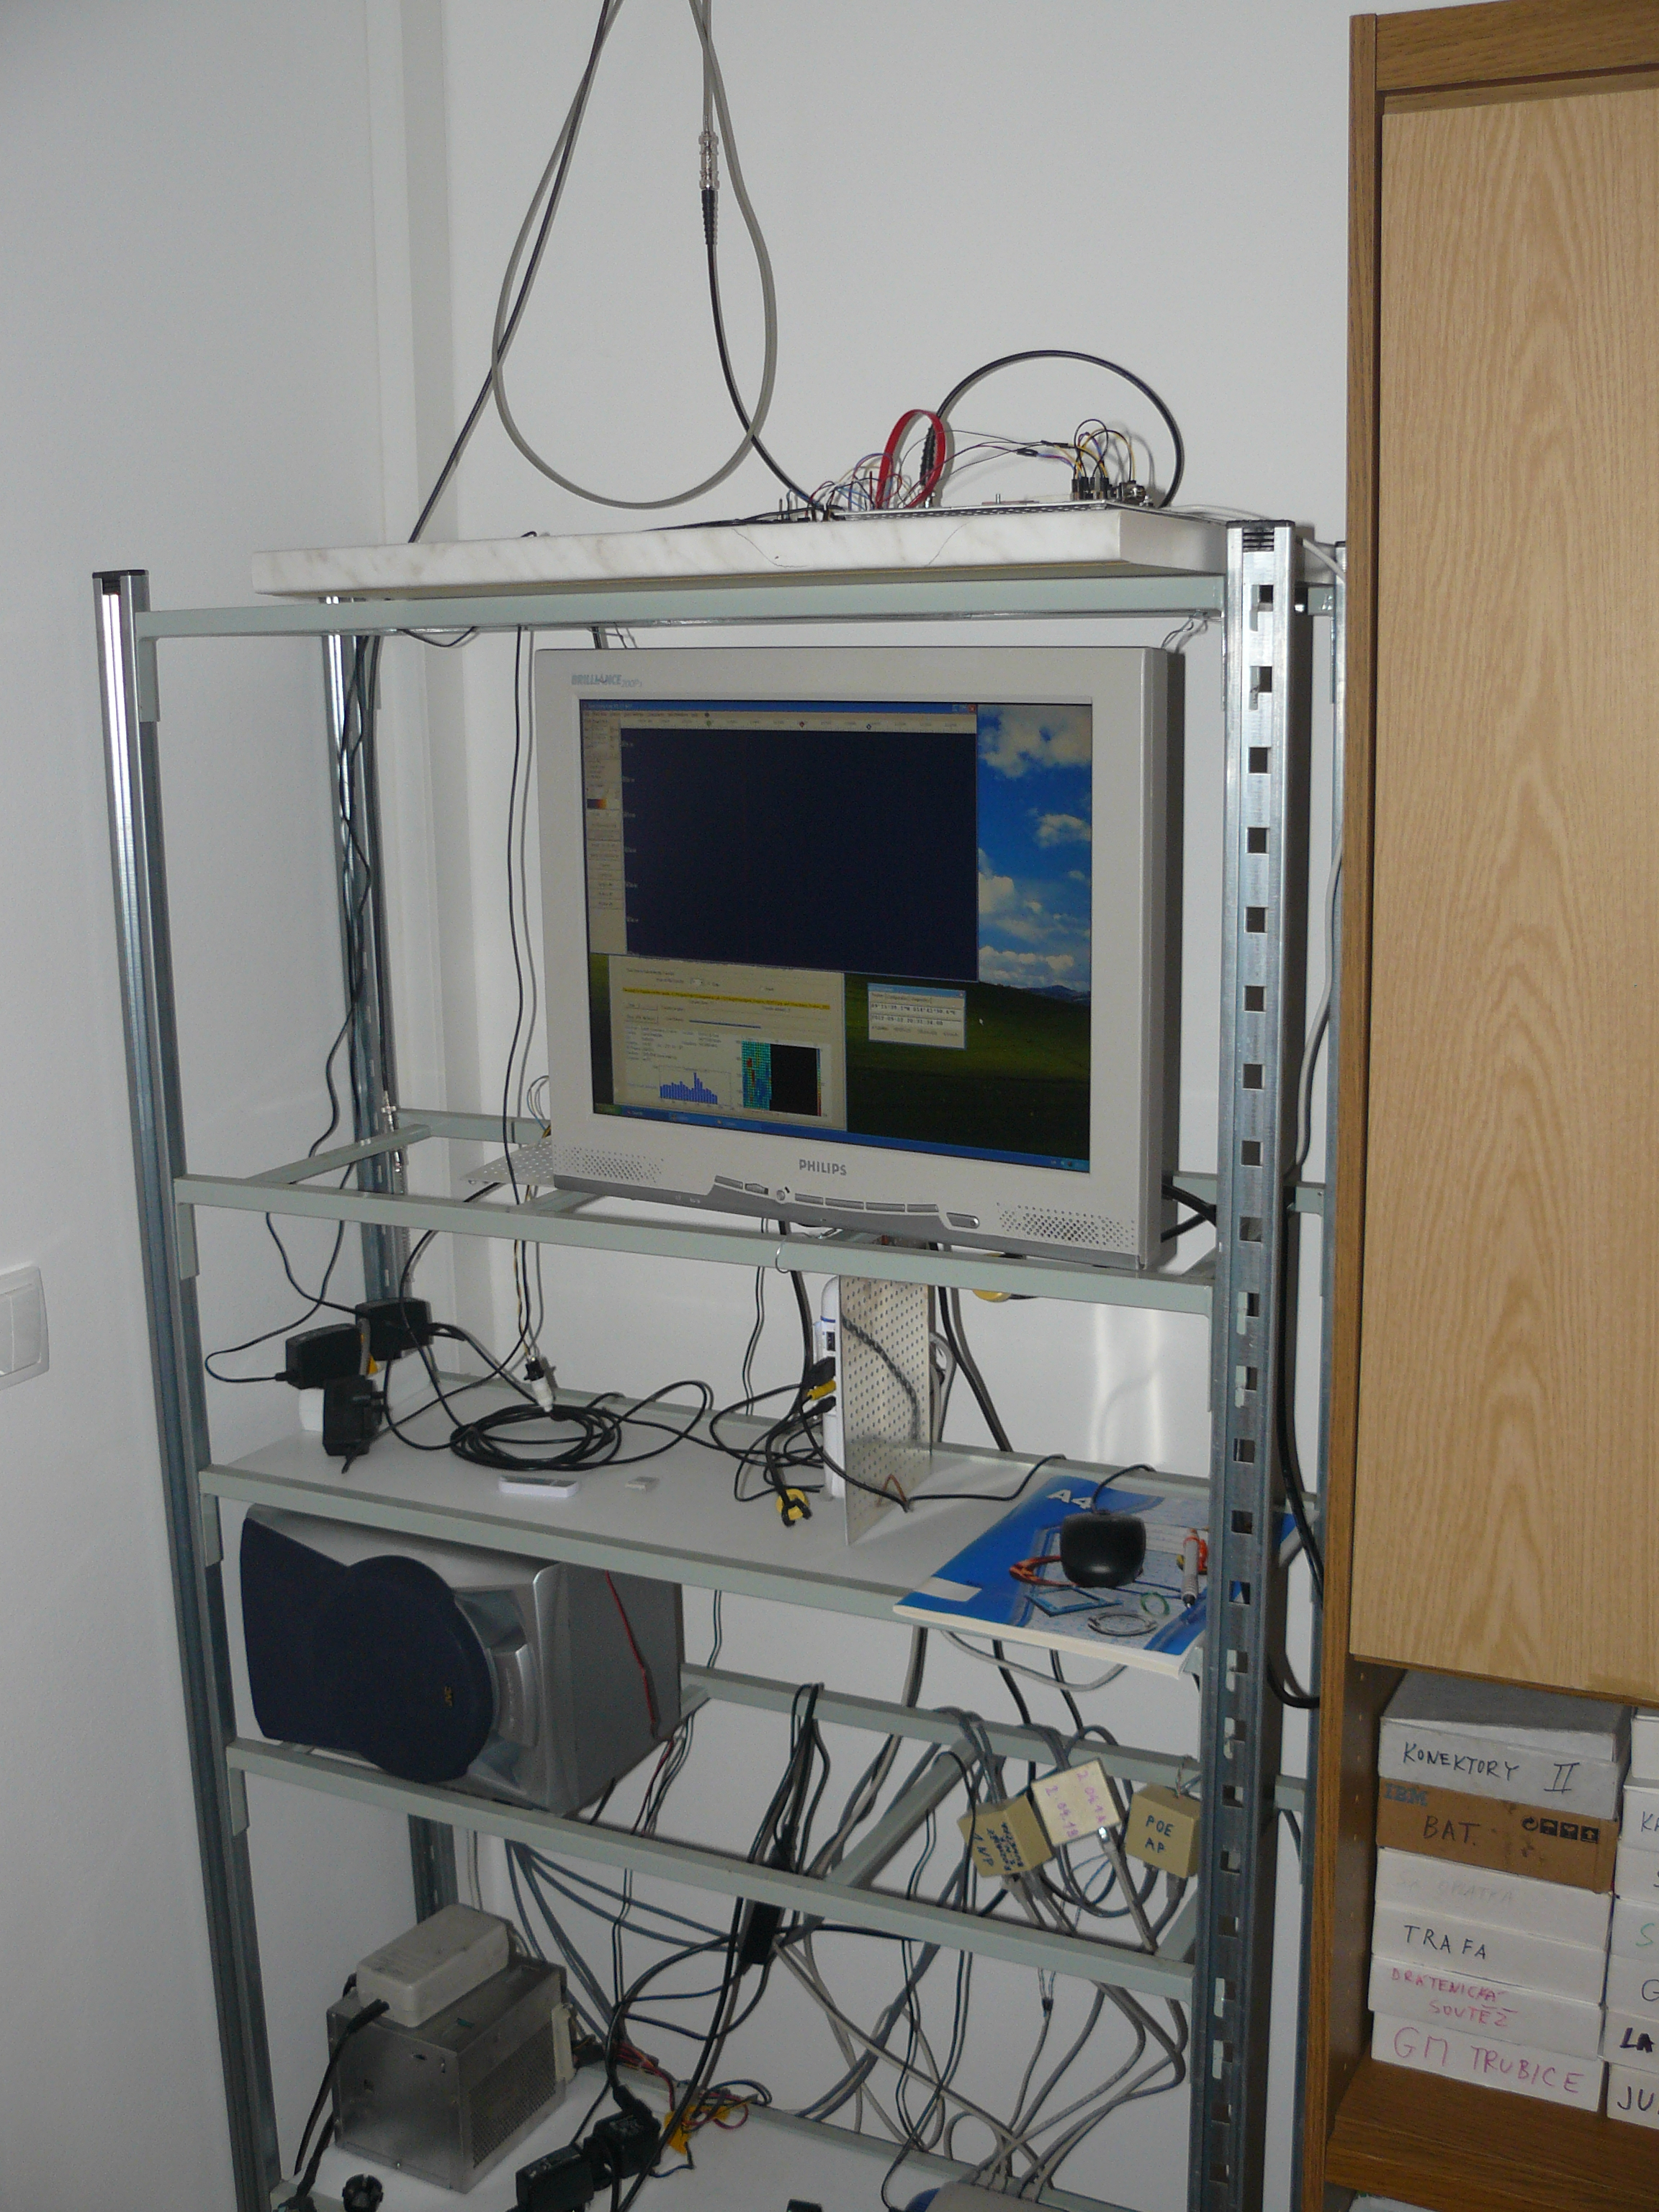
\includegraphics [width=80mm] {./img/meteor_detector_station.JPG} 
\end{center}
\end{figure}

\begin{figure} [b]

\includegraphics [width=25mm] {./img/SDRX01B_QRcode.png} 
\end{figure}

\newpage
\tableofcontents

\section{Technical parameters}
\begin{table}[htbp]
\begin{center}
\begin{tabular}{|c|c|p{5cm}|}
\hline
\multicolumn{1}{|c|}{Parametr} & \multicolumn{1}{|c|}{Hodnota} & \multicolumn{1}{|c|}{Poznámka} \\ \hline
Napájení analogových obvodů & $\pm$12V &  cca 35mA \\ \hline
Napájení digitálních obvodů & +5V &  300mA \\ \hline
Napájení předzesilovače  & 9-12V &  500 mA maximum \footnote{Chráněno vratnou PTC pojistkou 750mA na desce přijímače} \\ \hline
Frekvenční rozsah  & 0,5 - 200 MHz & Obvykle 143.05 MHz \\ \hline
Celkový zisk & 60-90 dB & Volitelně podle konfigurace LNA \footnote{Lze ovlivnit jumperem na desce přijímače}\\ \hline
Vlastní šumové číslo & $<$ 30 dB & \\ \hline
\end{tabular}
\end{center}
\end{table}

\newpage
\section{Princip rádiové detekce meteorů}

Nejznámější metodou radiové detekce meteorů je metoda označovaná, jako dopředný rozptyl. Tento princip využívá rozptylu rádiových vln na ionizované stopě meteoru. Zdrojem rádiových vln je v takovém případě již existující vysílač (historicky to byly například televizní, nebo rozhlasové vysílače), který je umístěný pokud možno pod radiovým horizontem přijímače, tak aby nebyla slyšitelná jeho přímá vlna, která by mohla zahltit detekční stanici příliš intenzivním signálem.  Rádiové vlny se pak odrážejí prakticky výhradně od ionizovaných stop během jejich vzniku a i při následné rekombinaci, to způsobuje vznik charakteristického signálu, který je pozorovatelný v blízkosti nosné frekvence vysílače. Většina těchto ionizovaných stop vzniká v horní atmosféře ve výškách okolo 100 $\pm$ 20 km.  

Přímý odraz od samotného meteoroidu není obvykle detekovatelný z několika důvodů, jednak materiál meteoroidu není obvykle dostatečně reflexivní pro radiové vlny a zároveň jeho rozměr je velmi malý (0.05 - 200mm) a je tedy zlomkem vlnové délky rádiových vln. Tato malá zrníčka prachu ale vstupují do horních vrstev atmosféry se supersonickými rychlostmi. Což způsobuje vznik rázové vlny, prudké ohřátí plynu a jeho ionizaci. Tato rázová vlna navíc dosahuje do velké vzdálenosti od samotného zrníčka minimálně jednotky metrů, což je již rozměr dostačující k interakci s radiovou vlnou. Ovšem vzhledem k supersonickým rychlostem pohybu meteoroidu má odražená vlna velký dopplerovský posuv a intenzita odrazu je navíc na začátku slabá, proto je v této fázi těžké odraz správně detekovat. Nicméně v zápětí se doplerovský posuv vlivem snížení rychlosti zmenšuje až k frekvenci vysílače, nebo i mírně pod ní. Pak je možné pozororovat relativně silný odraz. Tento jev se pak nazývá "head echo" a je způsoben odrazem signálu od čela plazmatického tubusu vznikajícího v atmosféře v těsné blízkosti meteoroidu. Je zřejmé, že tento jev nebude pozorovatelný naprosto vždy, neboť závisí na geometrii průletu meteoru vzhledem k vysílači a k detekční stanici. A v některých případech proto bude pozorován pouze odraz od stopy bez výrazných dopplerovských jevů. 

Při popisu principu této metody detekce se často můžeme setkat s pojmem meteorický radar.  Ovšem slovo RADAR je ve skutečnosti zkratka pro 'radio detection and ranging', ovšem vzdálenost a směr mohou být získána pouze z dat získaných ze skupiny přijímačů. Jedna přijímací stanice proto není případem radarového systému.  Samostatný přijímač je proto schopen pouze změřit četnosti meteoroidů vstupujících do atmosféry v prostoru osvětleném vysílačem. Některé další charakteristiky je sice možné získat zpětnou analýzou záznamů odrazů, ale zdánlivě jasné údaje, jako vazba mezi intenzitou odrazu a hmotností meteoroidu je komplikovaná problémy s neznámou polarizací signálu, trajektorií meteoru a pokrytím oblohy vysílačem.
    
Jednou z hlavních výhod rádiové detekce meteorů je fakt, že tato metoda funguje nezávisle na počasí, i jasu oblohy. A to jak ve dne, tak i v noci. Zvolením vhodné frekvence a výkonu vysílače je navíc možné detekovat i meteory, které by jinak byly příliš slabé k pozorování okem, nebo celooblohovou kamerou. Počty detekovaných rádiově detekovaných meteorů jsou proto obvykle řádově vyšší, než u optického pozorování. 
 
\section{Konstrukce detekční stanice}

This construction of radio meteor detector uses France GRAVES space-surveillance radar. The radar has transmitting power of several megawatts at frequency 143.05 MHz.   

Tato konstrukce rádiové detekčňí stanice využívá jako vysílače francouzský space-surveillance radar GRAVES určený k měření drah družic. Tento radar má výkon v řádu jednotek megawattů a vysílá na frekvenci 143.05 MHz.

\subsection{Antenna}
The detector station usually uses  modified ground plane antenna. Adjusted in angle of 30$^\circ$ to East this configuration seems to be optimal to detecting stations in the Czech Republic. 

\begin{figure} [htbp]
\begin{center}
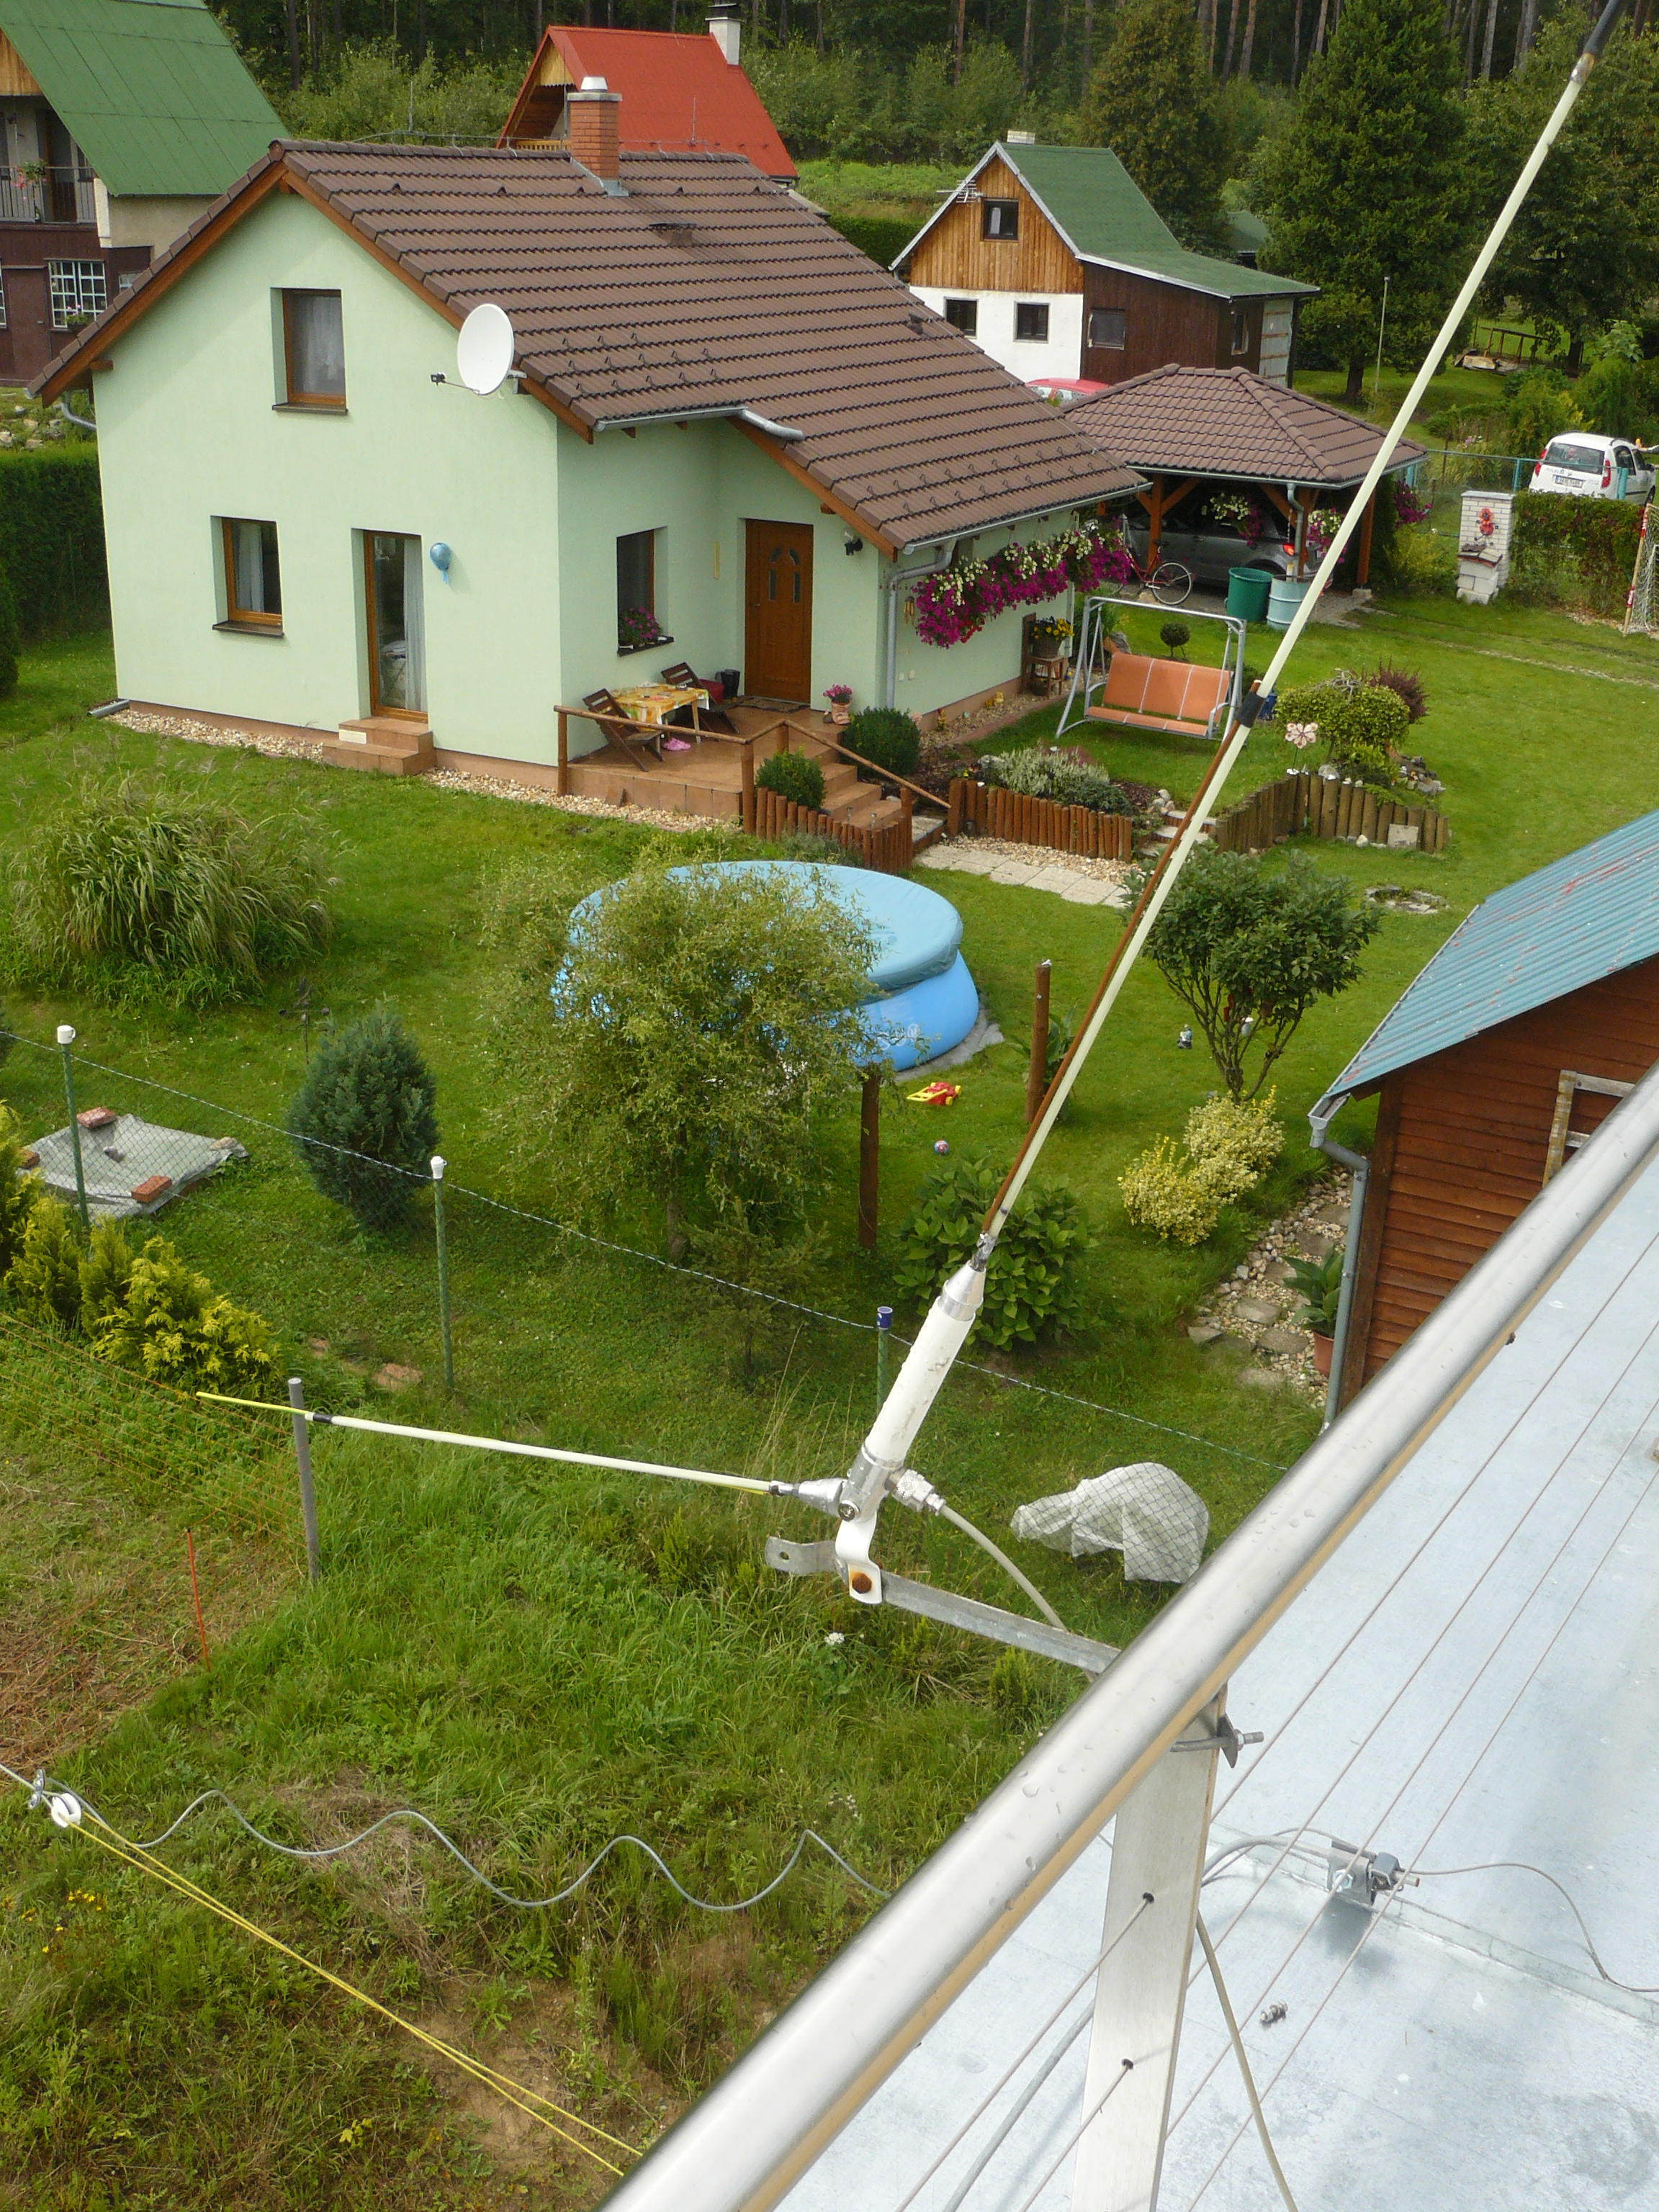
\includegraphics [width=80mm] {./img/GP143MHz.JPG} 
\end{center}
\caption{Antenna used at detection station}
\end{figure}

The received signal from antenna is amplified by specially constructed LNA. This step is needed for feeding the signal trough relative long (several metres) coax RG58. Construction of LNA01A is described on MLAB project site. 

\subsection{SDR receiver}

The SDR receiver used is MLAB system SDRX01B direct sampling receiver. This receiver has ideal performance for UHF and lower band radioastronomy.    So this receiver can be used even for radio meteor detection. 

\begin{figure} [htbp]
\begin{center}
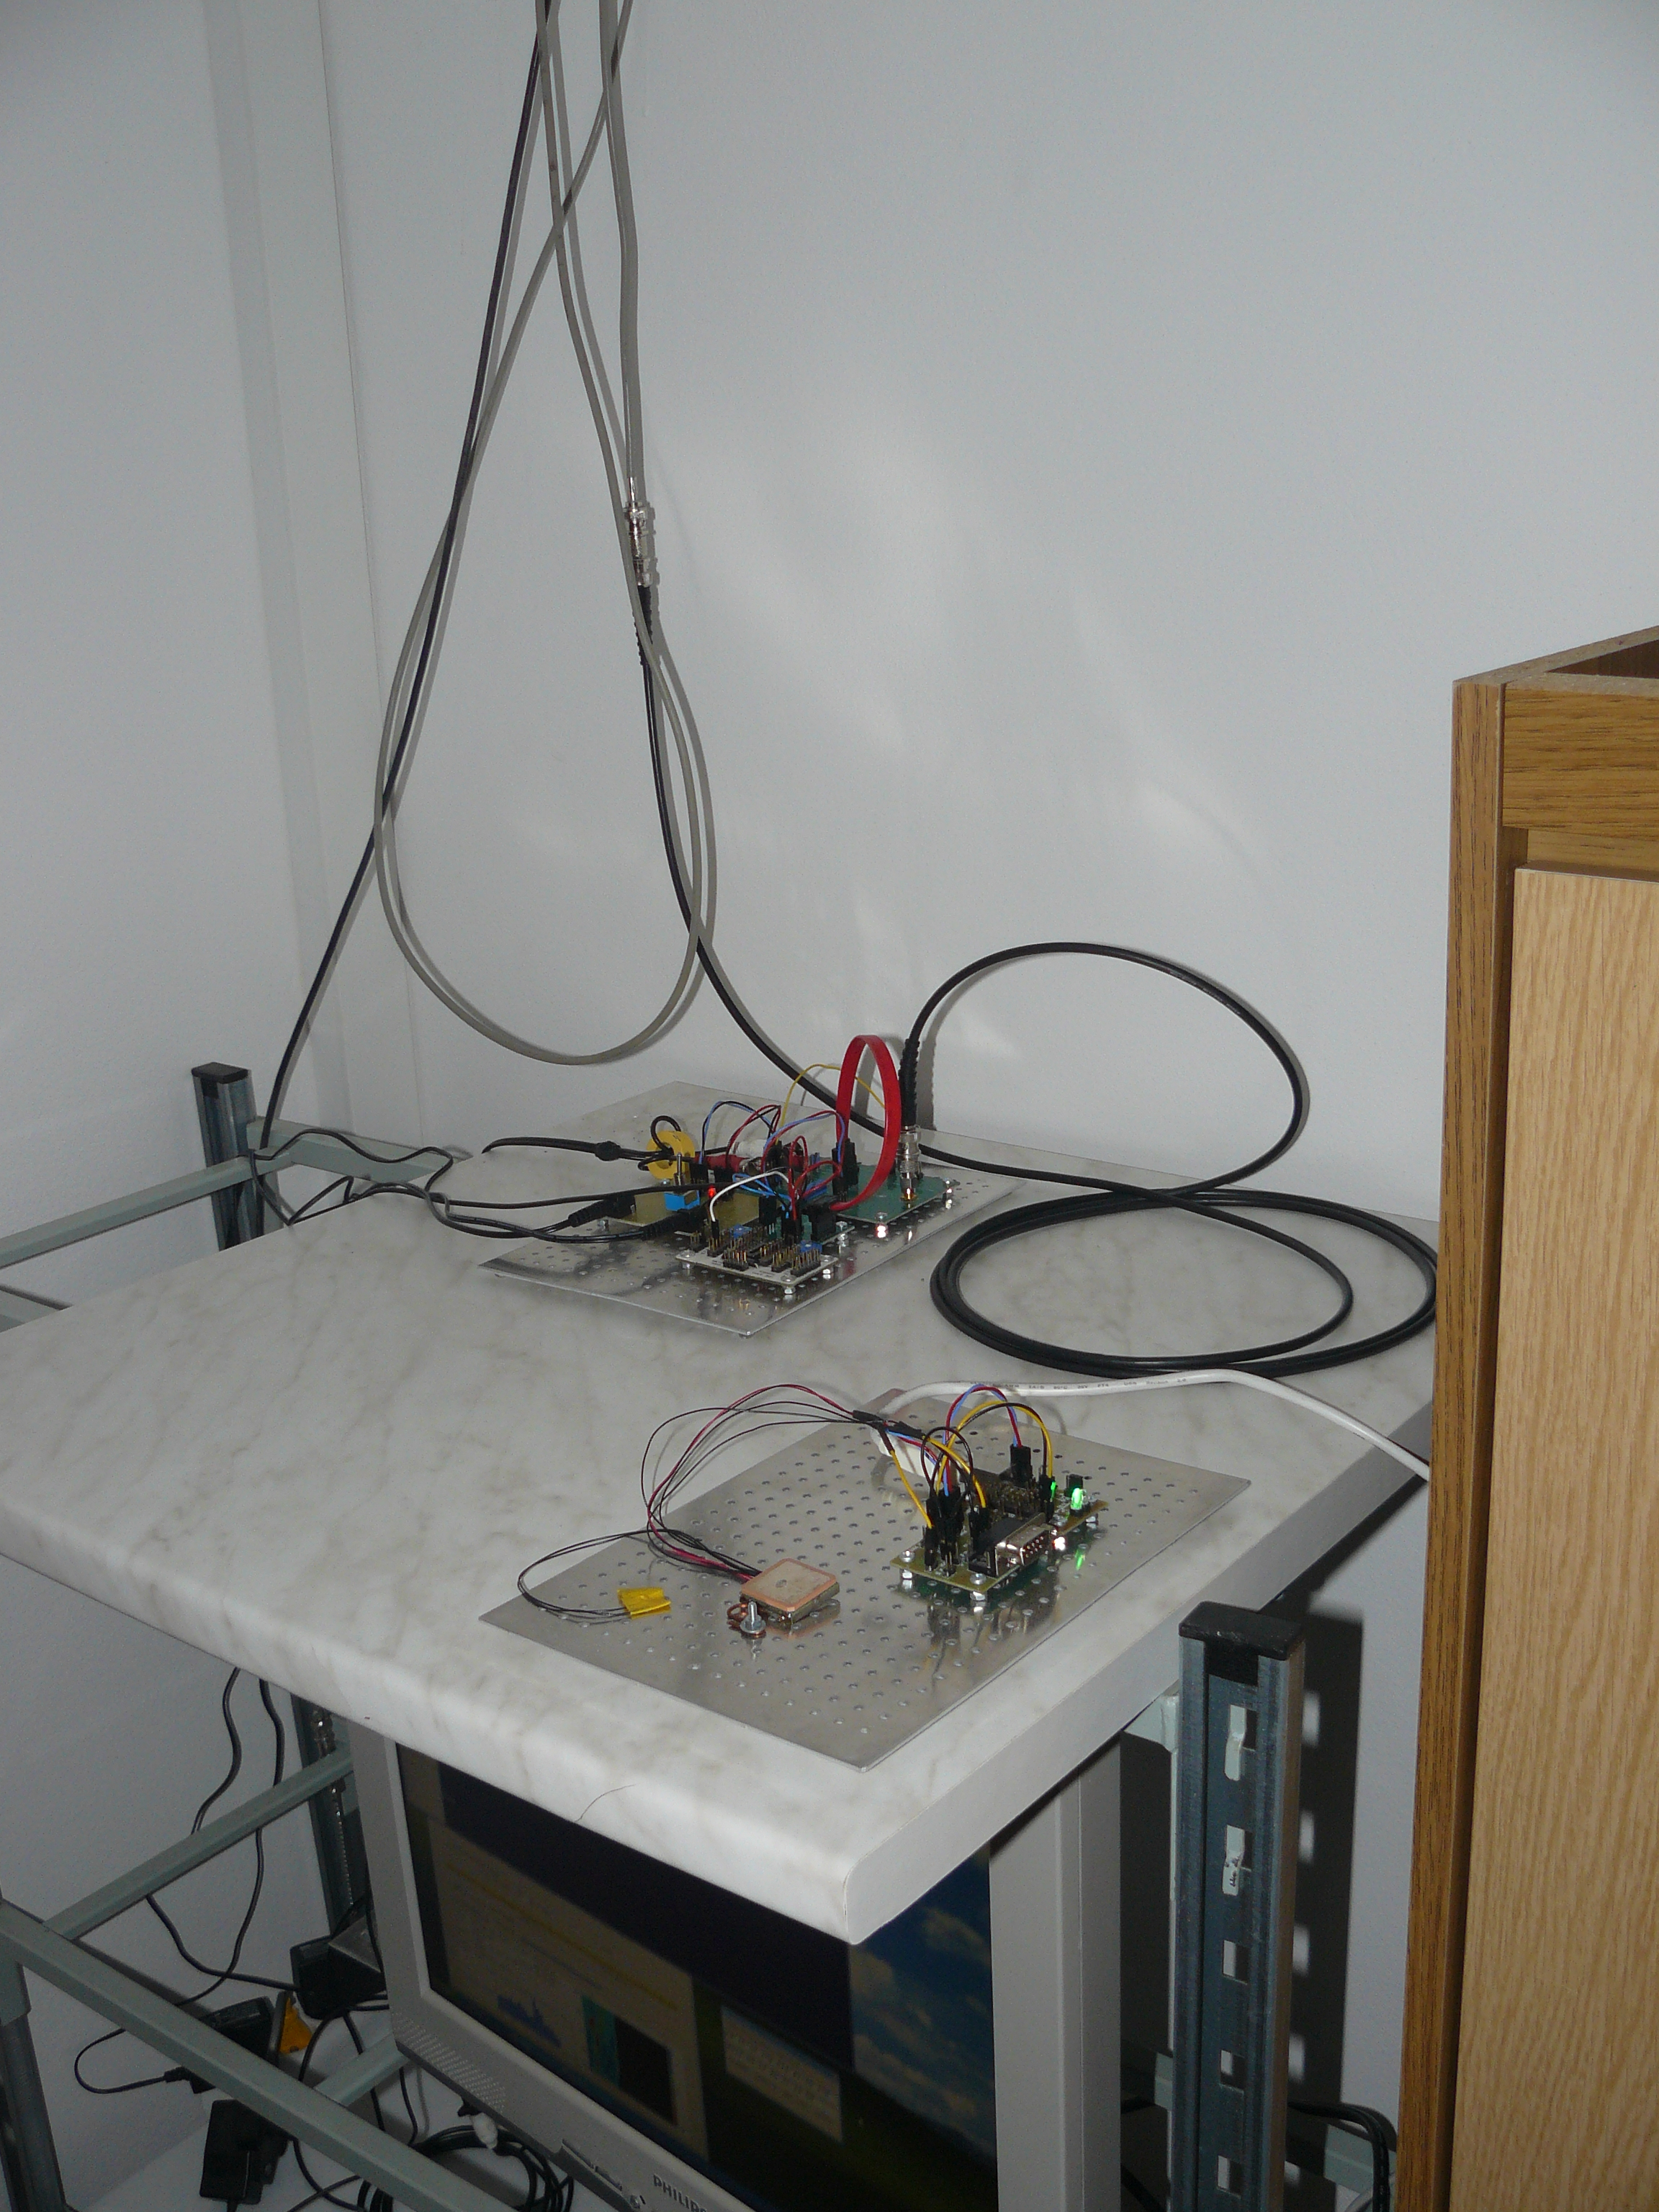
\includegraphics [width=80mm] {./img/meteor-detector_receiver.JPG} 
\end{center}
\caption{Example of meteor detector receiver setup}
\end{figure}


\begin{figure} [htbp]
\begin{center}
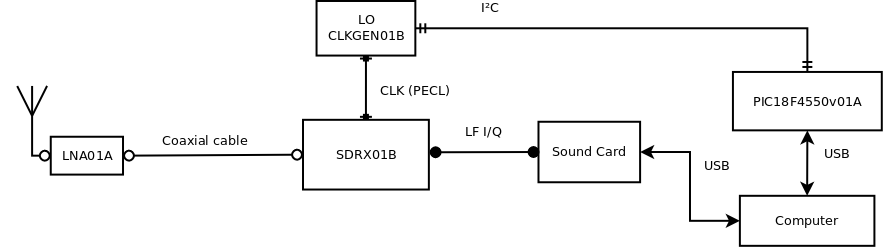
\includegraphics [width=150mm] {./img/RMDS01A_system.png} 
\end{center}
\caption{Schematic drawing of complete meteor detector}
\end{figure}


\subsection{Time synchronisation}

Time synchronisation has crucial importance in any modern science measurement. There is possibility of using many synchronisation techniques. Such as NTP or GPS (see for our article at  for our experiences)

Suggested method for time synchronisation of a measuring station depends on level of desired information which would be obtained from meteor reflection event.    

For example: If we need hour count data only. We can use PC system time without any synchronisation. But if we have one more station and we would like to compare data with another stations then NTP syncing would be good choice.  Highest level is trail parameters determination which need true radar signal processing  and most precise time synchronisation which could be achieved by GPS receiver.

\begin{figure}[htbp]
\begin{center}
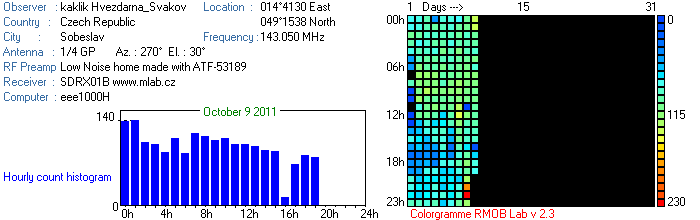
\includegraphics [width=150mm] {./img/colorgram.png} 
\end{center}
\caption{Example of measured hourly count of meteor showers}   
\end{figure}

\section{Software setup}

For simple PC based monitor station we are using SpectrumLab software with   our configuration and detection script. 

Local oscillator of SDRX01B is a CLKGEN01B module with frequency tuning controller  PIC18F4550v01A can be set up from PC or can be programmed for fixed start up frequency. If fixed start up frequency is correctly saved the only step for tuning the LO is provide power trough USB cable from PC and then press the RESET button of tuning microcomputer module. After that the LO shout be tuned on saved start up frequency. This frequency can be changed by   

\begin{thebibliography}{99}
\bibitem{Spectrum_lab}{Spectrum Lab} 
\href{http://www.qsl.net/dl4yhf/spectra1.html}{http://www.qsl.net/dl4yhf/spectra1.html}

\bibitem{Radio_meteor_detection}{Radio Meteor Detection} 
\href{http://www.gb2nlo.org/index.php/articles/meteordet}{http://www.gb2nlo.org/index.php/articles/meteordet}

\bibitem{meteor_distance}{Meteor distance parameters} 
\href{http://www.amsmeteors.org/richardson/distance.html}{http://www.amsmeteors.org/richardson/distance.html}




\end{thebibliography}
\end{document}